\documentclass[handout,compress]{beamer}

\usetheme[block=fill]{metropolis}

\usepackage{graphicx} % Allows including images
\usepackage{amsmath,amsfonts,amsthm,amssymb}
\usepackage{color}
\usepackage{xcolor,cancel}
%\setitemize{label=\usebeamerfont*{itemize item}%
%	\usebeamercolor[fg]{itemize item}
%	\usebeamertemplate{itemize item}}
\definecolor{mDarkBrown}{HTML}{604c38}
\definecolor{mDarkTeal}{HTML}{23373b}
\definecolor{mLightBrown}{HTML}{EB811B}
\definecolor{mMediumBrown}{HTML}{C87A2F}
\definecolor{mygreen}{HTML}{98C2B9}
\definecolor{myyellow}{HTML}{DFD79C}
\definecolor{myblue}{HTML}{8CA7CC}
\definecolor{kern}{HTML}{8CC2B7}

\usepackage{float}
\usepackage{framed}
\usepackage{epsfig}
\usepackage{graphicx}
\usepackage{subcaption}
\usepackage{ulem}
\usepackage{hhline}
\usepackage{multirow}
\usepackage{comment}   
\usepackage{bbm}
\usepackage{tikz}   
\usepackage{ulem}
\def\Put(#1,#2)#3{\leavevmode\makebox(0,0){\put(#1,#2){#3}}}
\newcommand*\mystrut[1]{\vrule width0pt height0pt depth#1\relax}
\newcommand{\eqdef}{\mathbin{\stackrel{\rm def}{=}}}


\newcommand{\bs}[1]{\boldsymbol{#1}}
\newcommand{\bv}[1]{\mathbf{#1}}
\newcommand{\R}{\mathbb{R}}
\newcommand{\E}{\mathbb{E}}

\DeclareMathOperator*{\argmin}{arg\,min}
\DeclareMathOperator*{\argmax}{arg\,max}
\DeclareMathOperator{\nnz}{nnz}
\DeclareMathOperator{\Var}{Var}
\DeclareMathOperator{\sinc}{sinc}
\DeclareMathOperator{\mv}{mv}
\DeclareMathOperator{\sgn}{sgn}
\DeclareMathOperator{\step}{step}
\DeclareMathOperator{\gap}{gap}
\DeclareMathOperator{\poly}{poly}
\DeclareMathOperator{\tr}{tr}
\DeclareMathOperator{\orth}{orth}
\newcommand{\norm}[1]{\|#1\|}
\captionsetup[subfigure]{labelformat=empty}
\captionsetup[figure]{labelformat=empty}
\DeclareMathOperator*{\lmin}{\lambda_{min}}
\DeclareMathOperator*{\lmax}{\lambda_{max}}

\newcommand{\specialcell}[2][c]{%
	\begin{tabular}[#1]{@{}c@{}}#2\end{tabular}}
\newcommand{\specialcellleft}[2][c]{%
	\begin{tabular}[#1]{@{}l@{}}#2\end{tabular}
}

\usepackage{tabstackengine}
\stackMath

\newtheorem{claim}[theorem]{Claim}


%----------------------------------------------------------------------------------------
%	TITLE PAGE
%----------------------------------------------------------------------------------------

\title{CS-UY 4563: Lecture 20 \\ Auto-encoders, Dimensionality Reduction, Principal Component Analysis}
\author{NYU Tandon School of Engineering, Prof. Christopher Musco}
\date{}

\begin{document}
	
	\begin{frame}
		\titlepage 
	\end{frame}
	
	\metroset{titleformat=smallcaps}
	
	\begin{frame}
		\small
		\frametitle{course logistics}
		{Convolutional neural net demo:} \texttt{demo\_classification.ipynb}.
		\begin{itemize}
			\item Classification on CIFAR 10 data set. 60k images, 10 classes.
			\item \textbf{You're going to want to use a GPU.} Easiest way to access more compute power is through Google Colab.
		\end{itemize}
	\begin{center}
		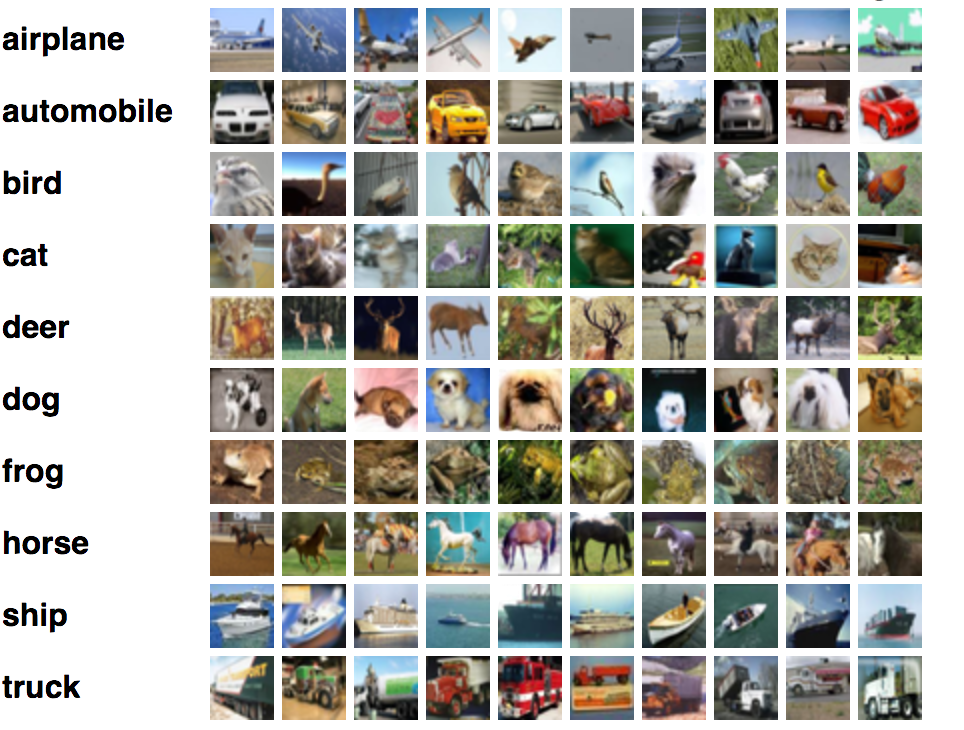
\includegraphics[width=.55\textwidth]{cifar10.png}
	\end{center}
	\end{frame}

\begin{frame}
	\frametitle{tricks of the trade}\small
	Beyond techniques already discussed (back-prop, batch gradient descent, adaptive learning rates) effectively training convolutional networks requires a lot of ``tricks''. In the demo we use:
	\begin{itemize}
		\item Batch normalization (accelerate training).
		\item Dropout (prevent over-fitting)
		\item Data-augmentation.
	\end{itemize}
\end{frame}

\begin{frame}
	\frametitle{batch normalization}
	\small Start with any neural network architecture:
	\begin{center}
		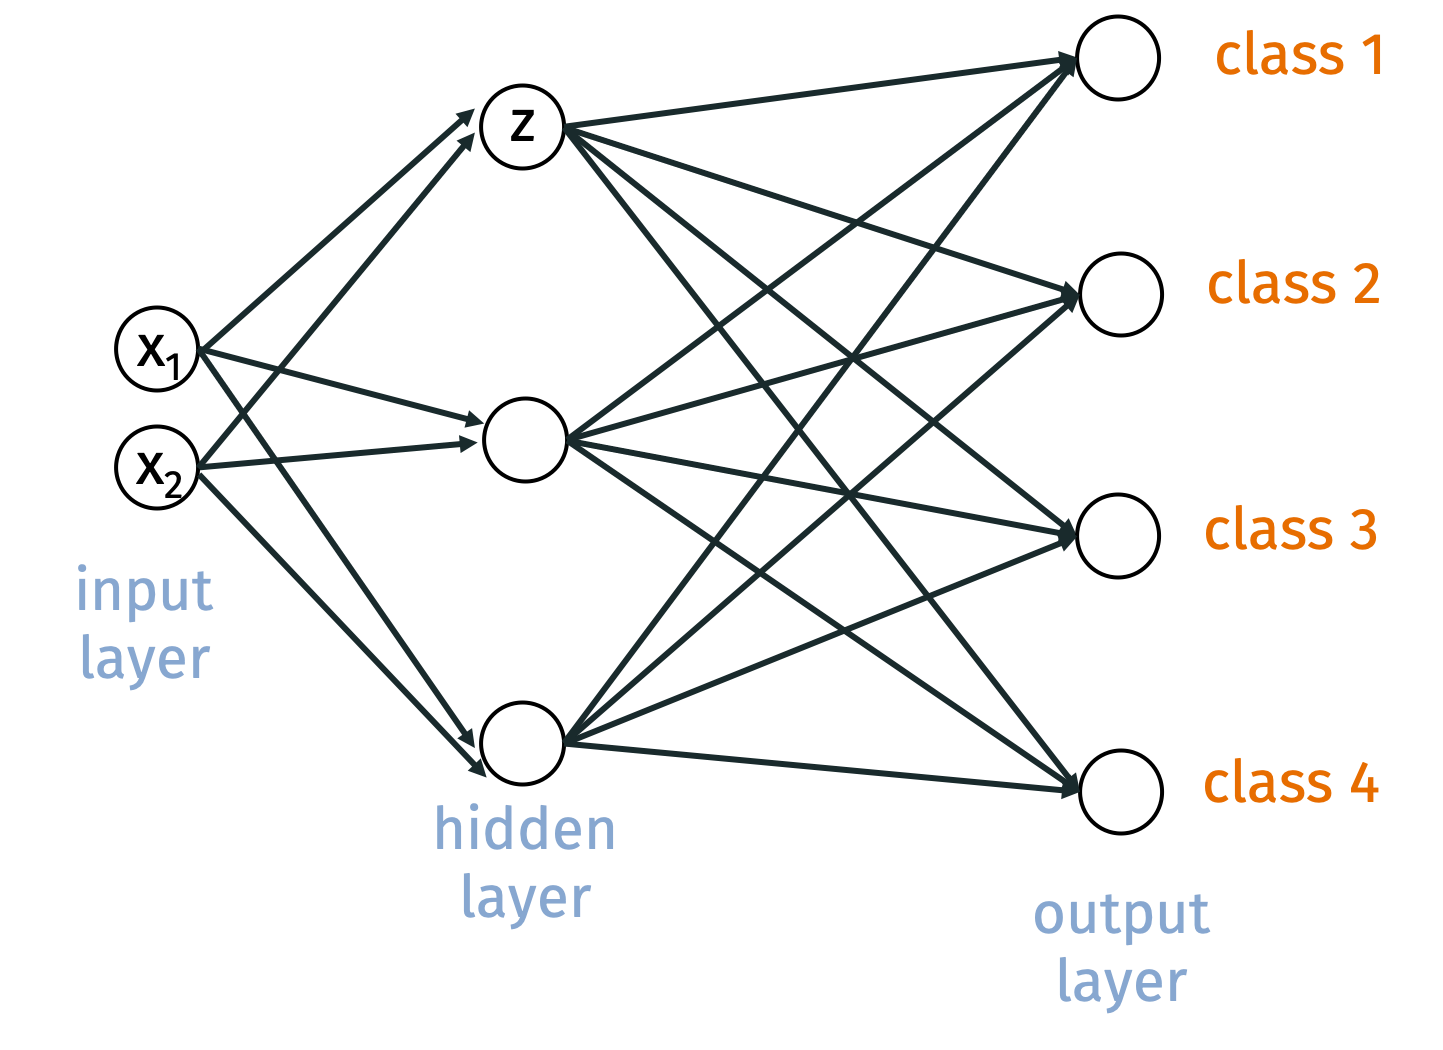
\includegraphics[width=.6\textwidth]{original_net.png}
	\end{center}
\vspace{-1em}
For input $\vec{x}$,
\begin{align*}
\bar{z} &= \vec{w}^T\vec{x} + b \\
z &= s(\bar{z})
\end{align*}
where $\vec{w}$, $b$, and $s$ are weights, bias, and non-linearity.
\end{frame}

\begin{frame}
	\frametitle{batch normalization}
	$\bar{z}$ is a function of the input $\vec{x}$. We can write it as $\bar{z}(\vec{x})$. Consider the mean and standard deviation of the hidden variable over our entire dataset $\vec{x}_1\ldots, \vec{x}_n$: 
	\begin{align*}
		\mu = \frac{1}{n}\sum_{j=1}^n \bar{z}(\vec{x}_j)\\
		\sigma^2 = \frac{1}{n}\sum_{j=1}^n (\bar{z}(\vec{x}_j) - \mu)^2
	\end{align*}
	Just as normalization (mean centering, scaling to unit variance) is sometimes used for \emph{input features}, batch-norm applies normalization to \emph{learned features}.
\end{frame}

\begin{frame}
	\frametitle{batch normalization}
	\small Can add a batch normalization layer after any layer:
	\begin{center}
		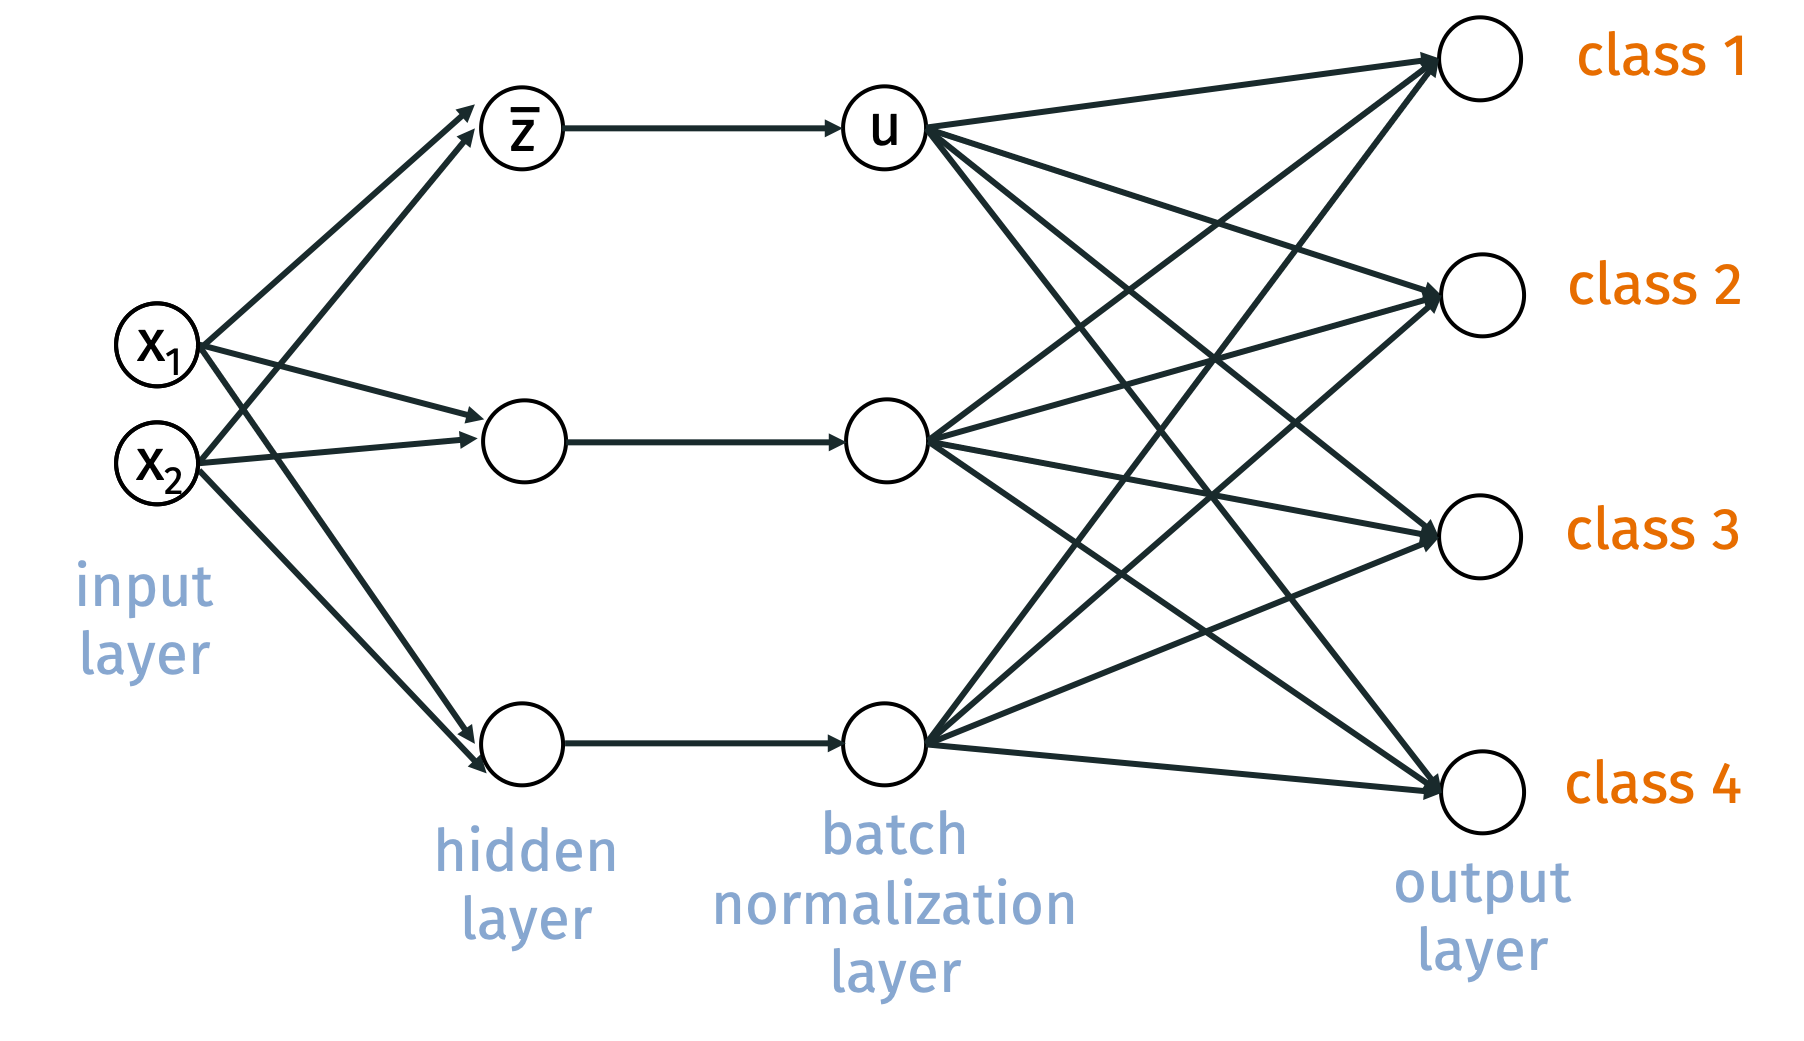
\includegraphics[width=.6\textwidth]{batch_norm.png}
	\end{center}
	\vspace{-1em}
	\begin{align*}
	\bar{u} &= \frac{\bar{z} - \mu}{\sigma} \\
	u &= s(\gamma \cdot \bar{u} + c).
	\end{align*}
	Where $\gamma$ and $c$ are \textbf{learned parameters}. Has the effect of mean-centering/normalizing $\bar{z}$, and then mapping back to have a new mean and new standard deviation.
\end{frame}

\begin{frame}
	\frametitle{batch normalization}
	\small
	\text{Proposed in 2015}: ``Batch Normalization: Accelerating Deep Network Training by Reducing Internal Covariate Shift'', Ioffe, Szegedy.
	\begin{center}
		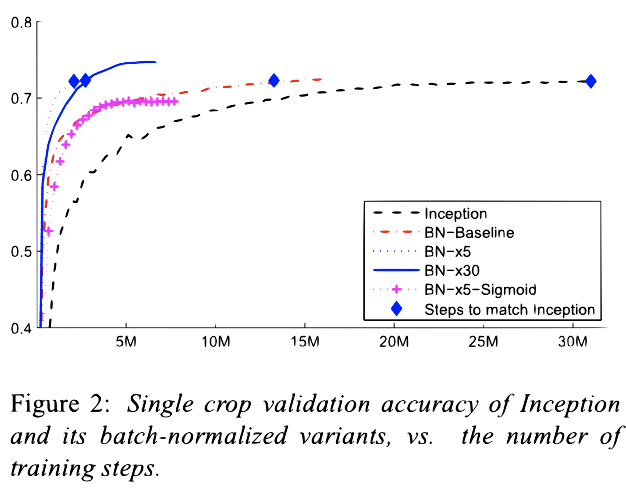
\includegraphics[width=.5\textwidth]{batch_norm_speed.png}
	\end{center}
	Doesn't change the expressive power of the network, but allows for significant convergence acceleration. Authors and others have good intuition for why: happy to discuss this more offline.
\end{frame}

\begin{frame}
	\frametitle{dropout}
	\small
	\text{Proposed in 2012}: ``Dropout: A Simple Way to Prevent Neural Networks from
	Overfitting'', Srivastava et al.
	\begin{center}
		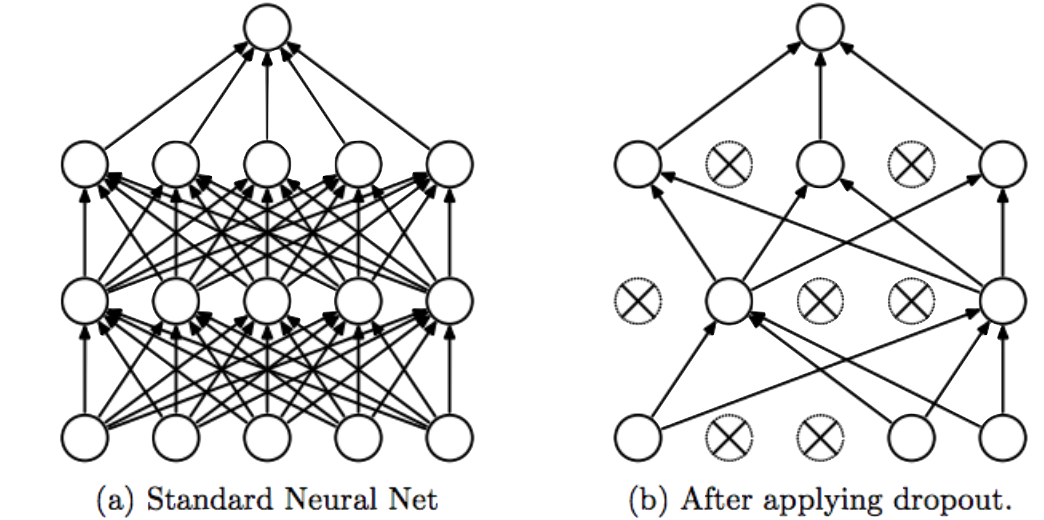
\includegraphics[width=.5\textwidth]{dropout.png}
	\end{center}
	During training, ignore a random subset of neurons during each gradient step. Select each neuron to be included independently with probability $p$ (typically $p \approx .5$). During testing, no dropout is used.
\end{frame}

\begin{frame}
	\frametitle{dropout}
	\small
	\begin{itemize}
		\item Only used on fully connected layers.
		\item Simultaneously performs model regularization (model simplification) and model averaging.
		\item Has become less important in modern CNNs (convolutional neural nets) as the final fully connected layers become less important. But still a very helpful technique to know about!
	\end{itemize}
	\begin{center}
	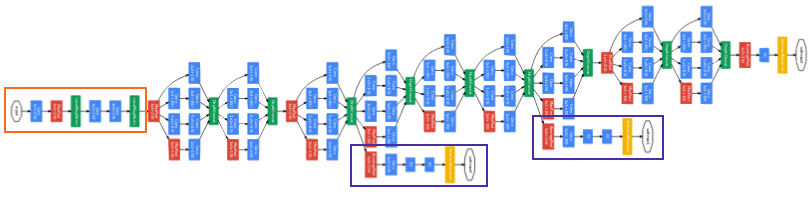
\includegraphics[width=.8\textwidth]{inception.png}
	\end{center}
\end{frame}


\begin{frame}
	\frametitle{data augmentation}
	\small
	Great general tool to know about. \textbf{Main idea:}
	\begin{itemize}
		\item More training data typically leads to a more accurate model.
		\item Artificially enlarge training data with simple transformations.
	\end{itemize}
\vspace{-1em}
	\begin{center}
	\includegraphics[width=.5\textwidth]{augmentation.png}\includegraphics[width=.48\textwidth]{augmentation2.png}
	\end{center}
\vspace{-1em}
Take training images and randomly shift, flip, rotate, skew, darken, lighten, shift colors, etc.  to create new training images. \textbf{Final classifier will be more robust to these transformations.}
\end{frame}

\begin{frame}
	\frametitle{one-shot learning}
	\small
	What if you want to apply deep convolutional networks to a problem where you do not have a lot of \textbf{labeled data} in the first place?
	\begin{center}
		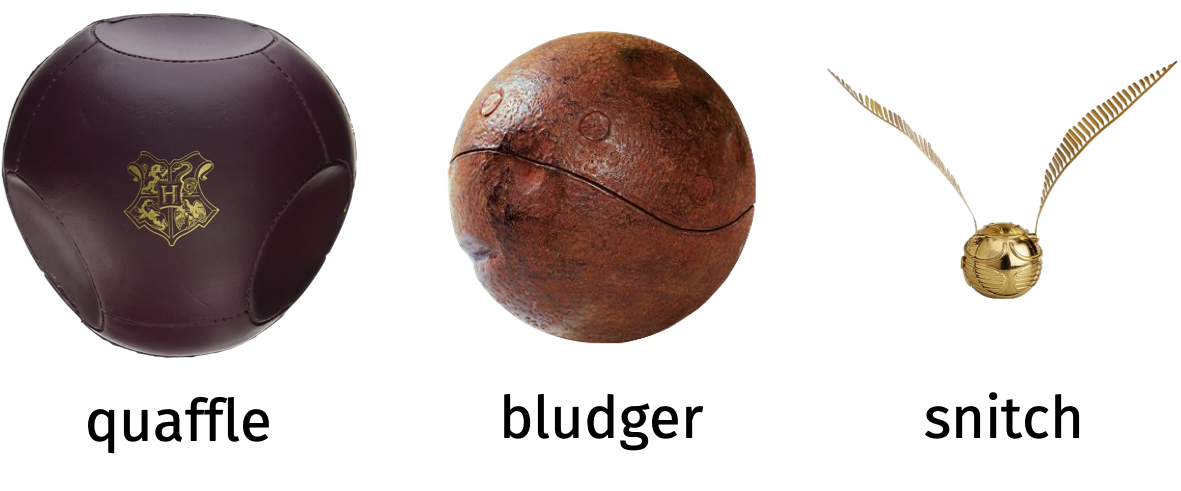
\includegraphics[width=.7\textwidth]{hp.png}
		
		\textbf{Example:} Classify images of different Quidditch balls.	
	\end{center}
\end{frame}

\begin{frame}
	\frametitle{one-shot learning}
	A human could probably achieve near perfect classification accuracy even given access to a \textbf{single labeled example} from each class:
	\begin{center}
		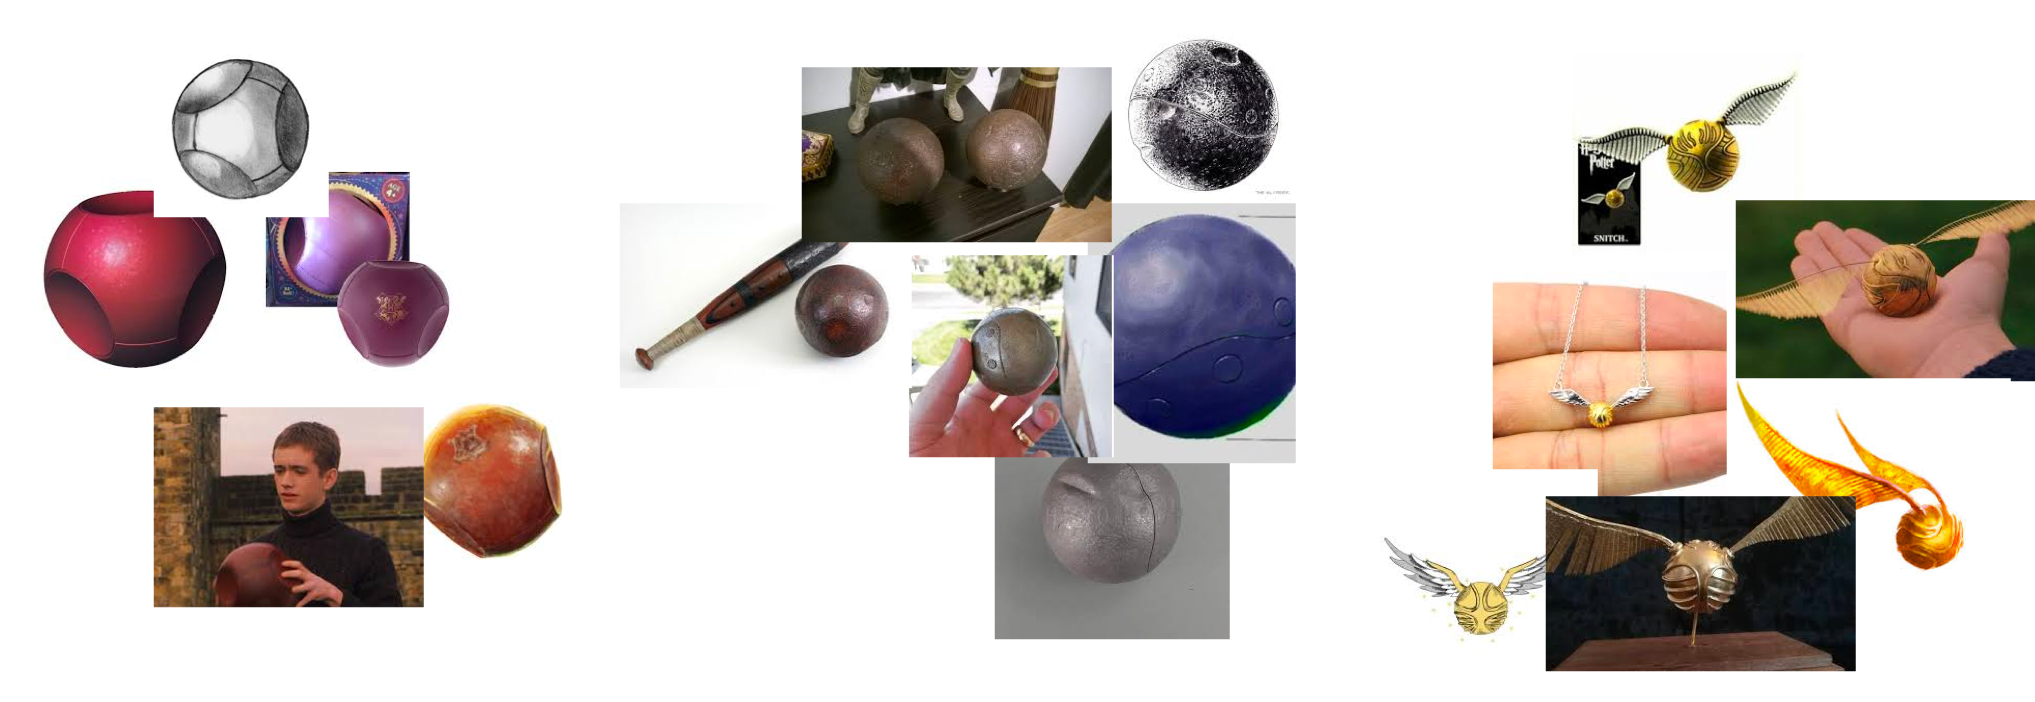
\includegraphics[width=\textwidth]{one_shot.png}
	\end{center}
	\textbf{Major question in ML:} How? Can we design ML algorithms which can do the same?
\end{frame}

\begin{frame}
	\frametitle{transfer learning}
	Transfer knowledge from one task we already know how to solve to another.
	\begin{center}
		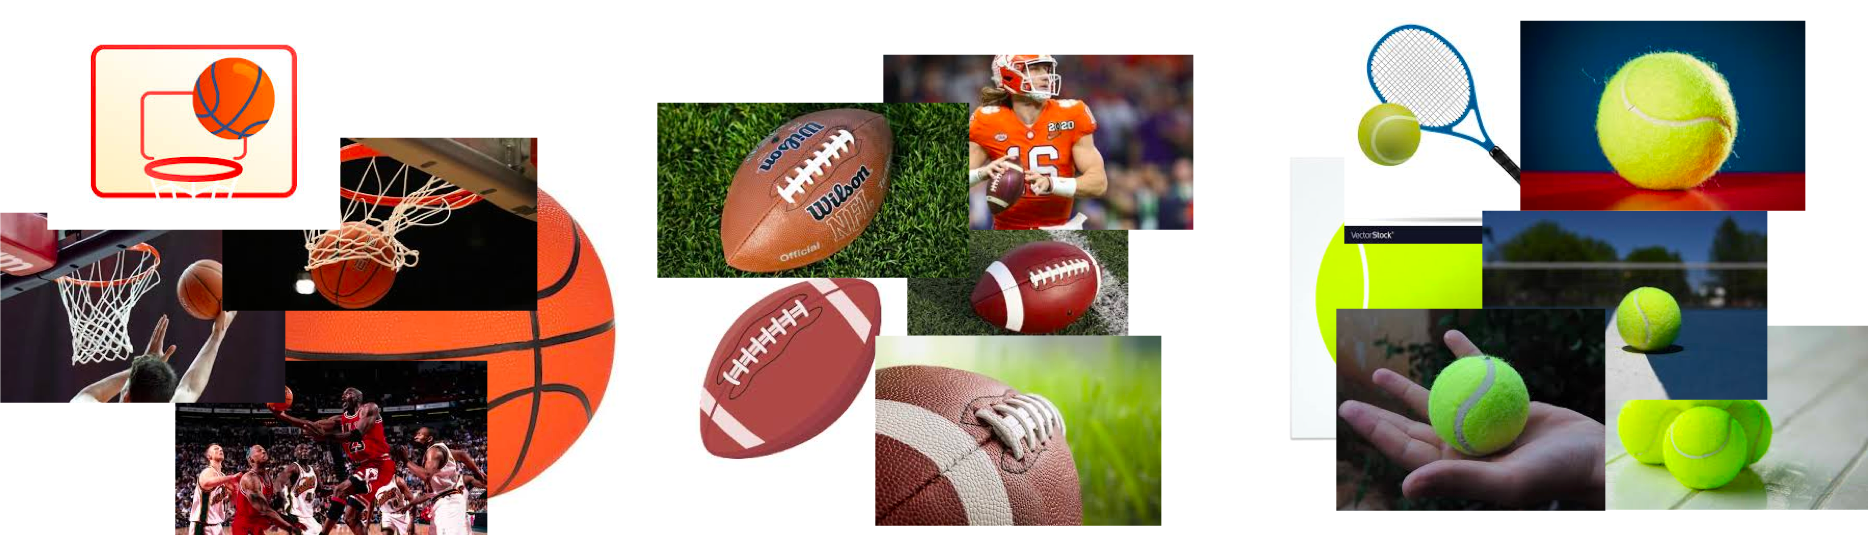
\includegraphics[width=\textwidth]{regular_balls.png}
	\end{center}
For example, we have learned from past experience that balls used in sports have consistent shapes, colors, and sizes. These \emph{features} can be used to distinguish balls of different type. 
\end{frame}

\begin{frame}
	\frametitle{feature learning}
	Examples of possible high-level features a human would learn:

		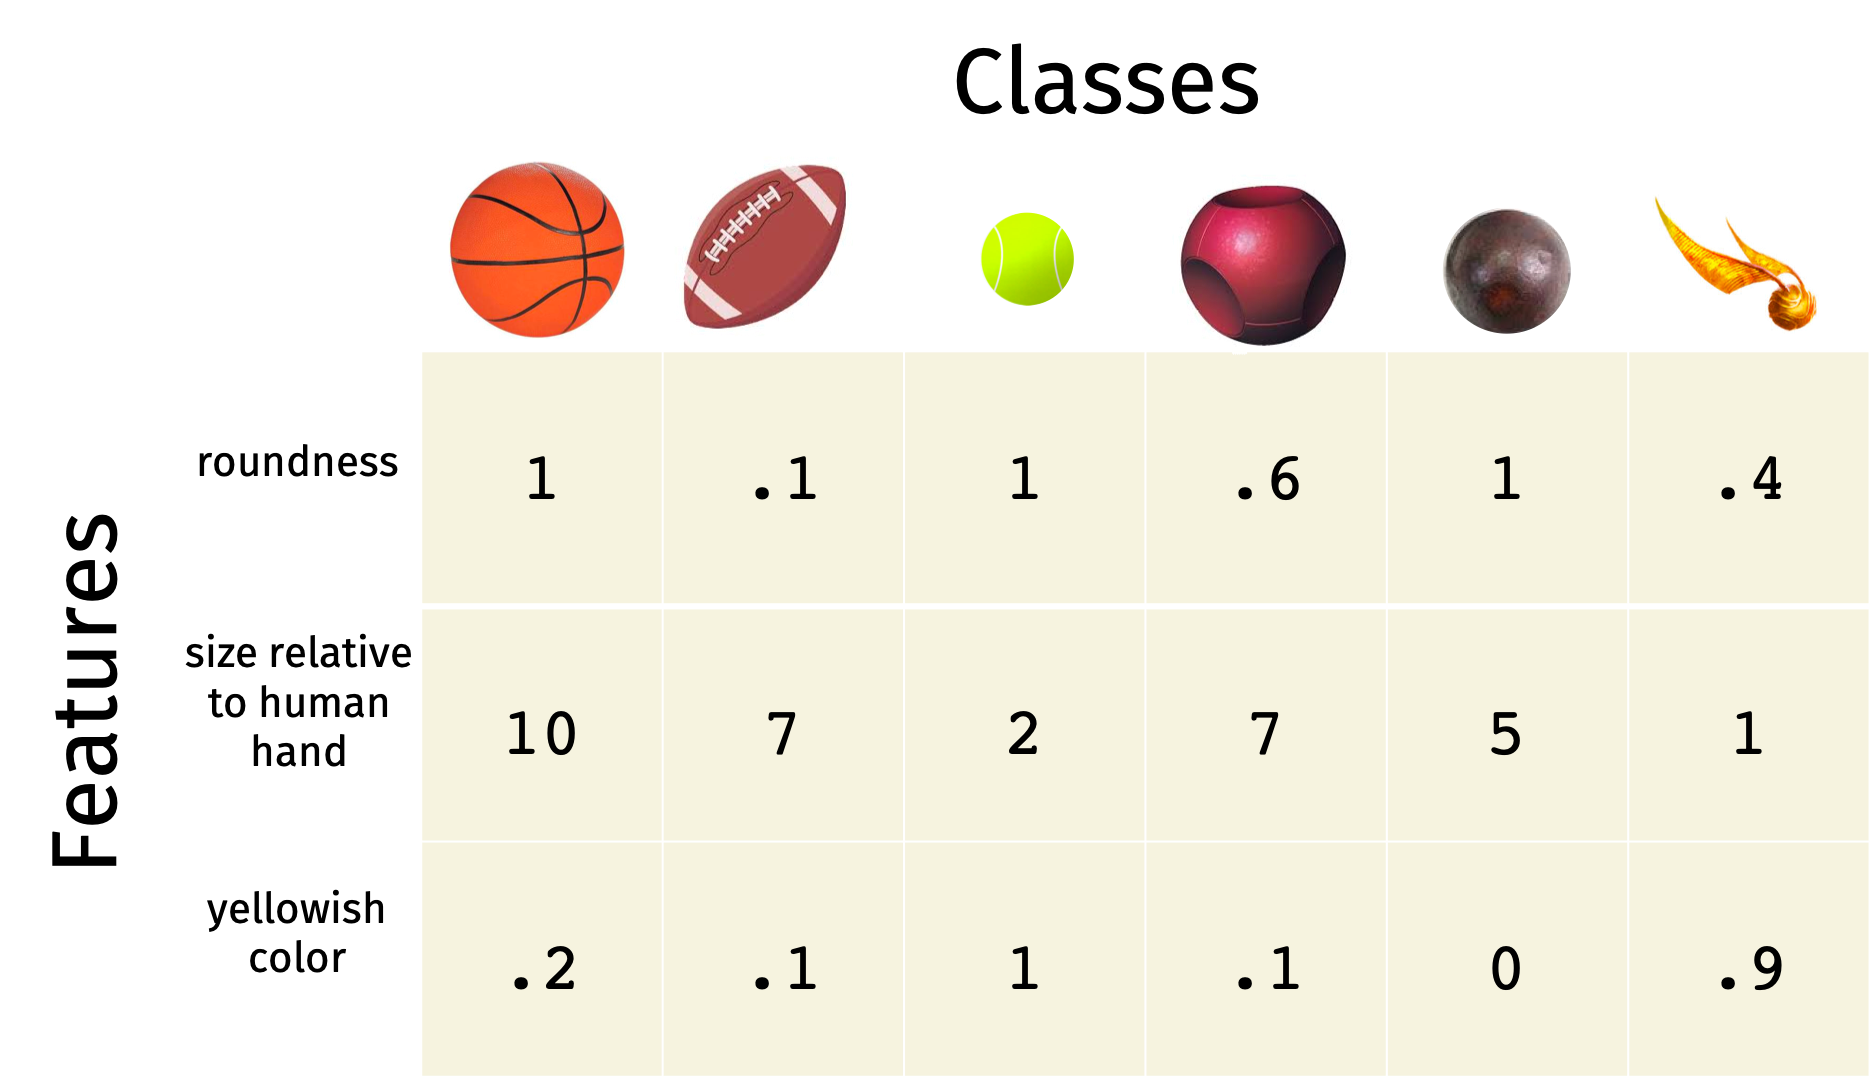
\includegraphics[width=.8\textwidth]{highlevel_features.png}
\end{frame}

\begin{frame}
	\frametitle{feature learning}
	If these features are highly informative (i.e. lead to highly separable data) few training examples are needed to learn.
	\begin{center}
		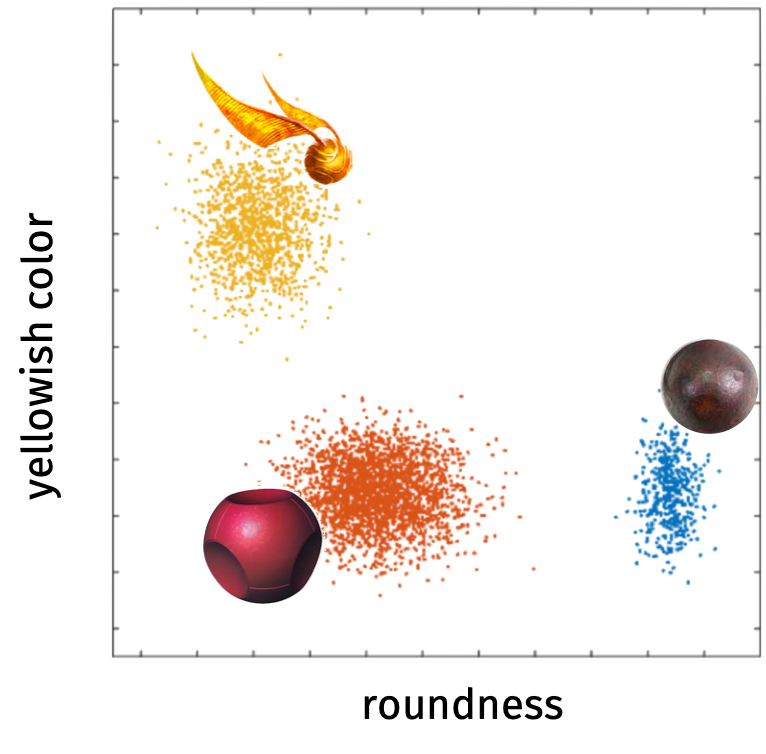
\includegraphics[width=.4\textwidth]{very_sep.png}
	\end{center}
Might suffice to classify ball using nearest training example in feature space, even if just a handful of training examples.
\end{frame}

\begin{frame}
	\frametitle{transfer learning}
	\textbf{Empirical observation:} Features learned when training models like deep neural nets seem to capture exactly these sorts of high-level properties. 
	\begin{center}
		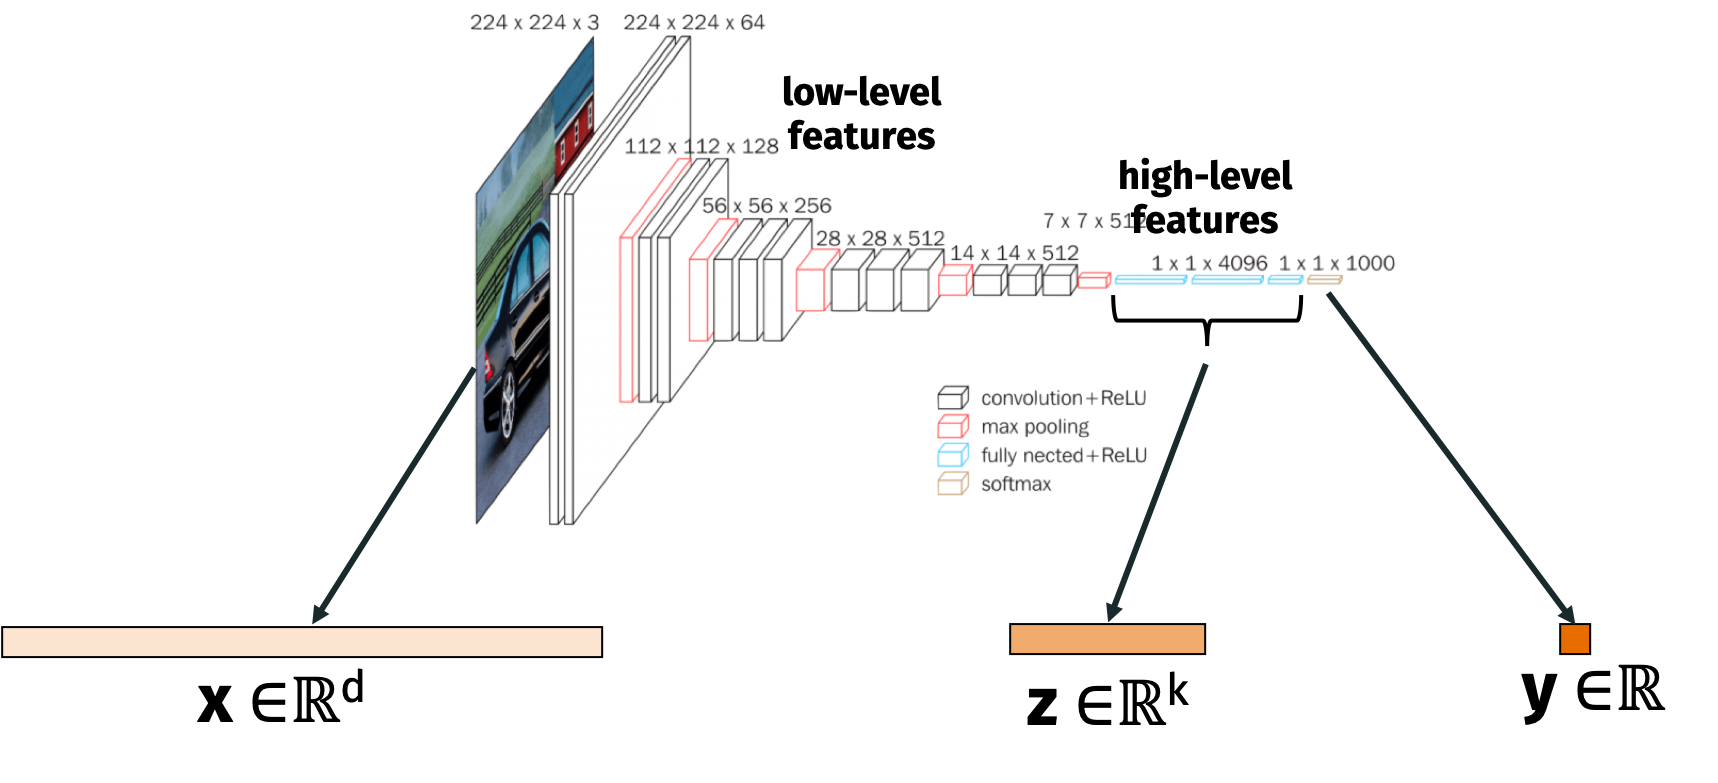
\includegraphics[width=\textwidth]{transfer_abstract.png}
	\end{center}
	Even if we can't put into words what each feature in $\vec{z}$ means...
\end{frame}

\begin{frame}
	\frametitle{transfer learning}
	\small
	This is now a common technique in computer vision:
	\begin{enumerate}
		\item Download network trained on large image classification dataset (e.g. Imagenet).
		\item Extract features $\vec{z}$ for amy new image $\vec{x}$ by running it through the network up until layer before last.
		\item Use these features in a simpler machine learning algorithm that requires less data (nearest neighbor, logistic regression, etc.).
	\end{enumerate}
This approach has even been used on the quidditch problem: \url{github.com/thatbrguy/Object-Detection-Quidditch}
\end{frame}

\begin{frame}
	\frametitle{unsupervised feature learning}
	\textbf{Transfer learning:} Lots of labeled data for one problem makes up for little labeled data for another.
	\begin{center}
		\textbf{What if we don't even have much labeled data for irrelevant classes?}
	\end{center} 
How to extract features in a data-driven way from \emph{unlabeled data} is one of the central problems in \textbf{unsupervised learning}.

\textbf{\alert{Unsupervised}} and \textbf{\alert{semi-supervised}} learning will be the main topics of the next 2 weeks.
\end{frame}

\begin{frame}
	\frametitle{supervised vs. unsupervised learning}
	\begin{itemize}
		\item \textbf{Supervised learning:} \emph{All} input data examples come with targets/labels. What machines are good at now.
		\item \textbf{Unsupervised learning:} \emph{No} input data examples come with targets/labels. Interesting problems to solve include clustering, anomaly detection, semantic embedding, etc.
		\item \textbf{Semi-supervised learning:} \emph{Some} (typically very few) input data examples come with targets/labels. What human babies are really good at, and we would love to make machines better at.
	\end{itemize}
\end{frame}


\begin{frame}
	\frametitle{transfer learning}
	\textbf{Back to the problem at hand:} Want to extract meaningful features from an already trained neural network.
	\begin{center}
		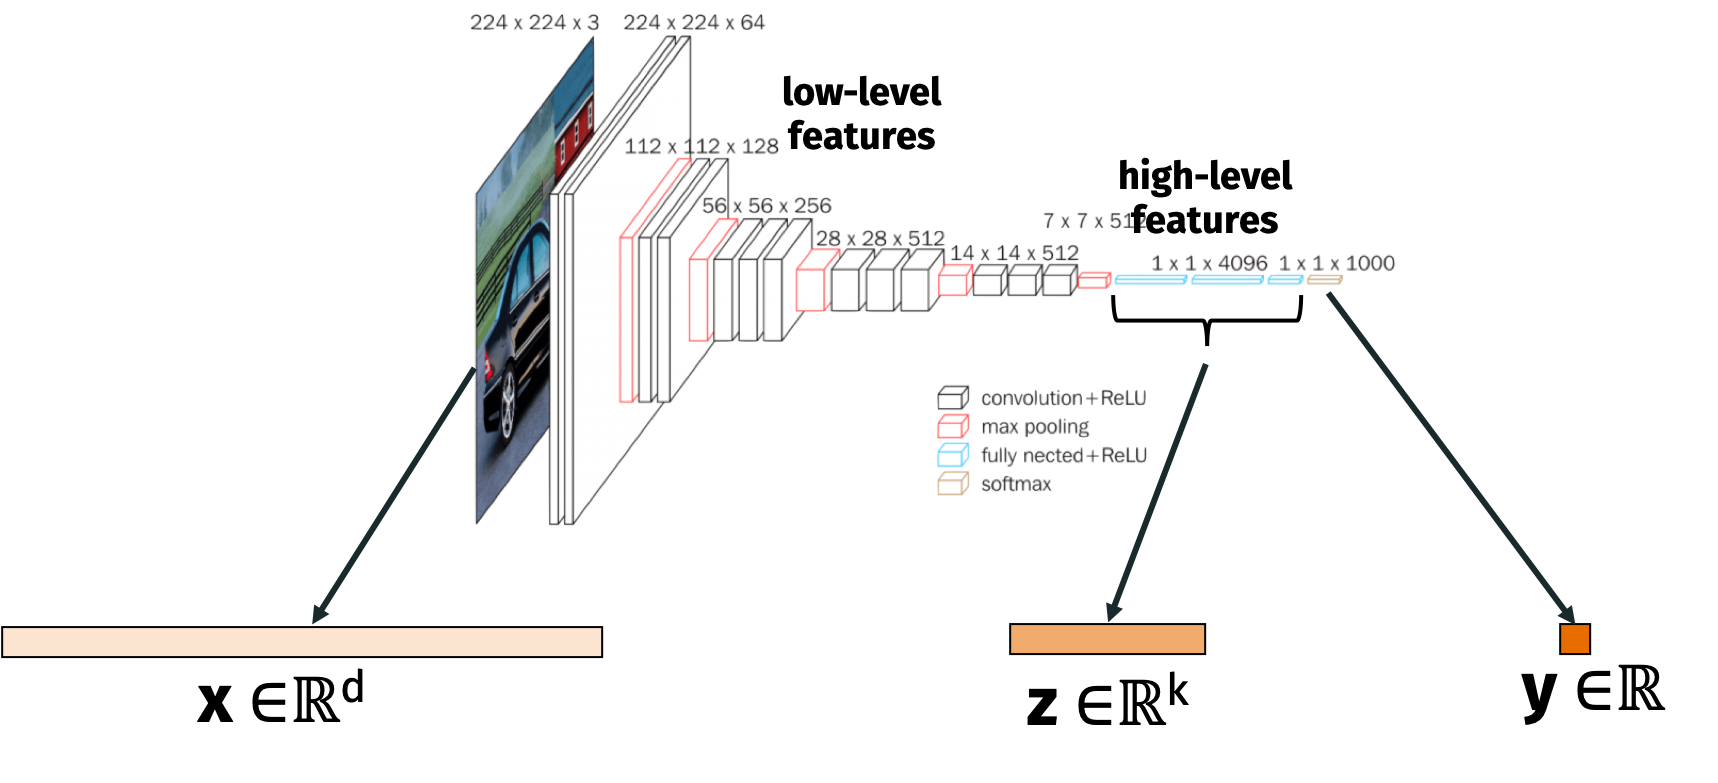
\includegraphics[width=\textwidth]{transfer_abstract.png}
	\end{center}
\end{frame}


\begin{frame}
	\frametitle{autoencoder}
	\textbf{Simple but clever idea:} If we have inputs $\vec{x}_1,\ldots, \vec{x}_n \in \R^d$ but no targets $y_1, \ldots, y_n$ to learn, just \emph{make the inputs the targets}. 
	\begin{itemize}
		\item Let $f_{\vec{\theta}}: \R^d \rightarrow \R^d$ be our model.
		\item Let $L$ be a loss function. E.g. squared loss: $L_{\vec{\theta}}(\vec{x}) = \|\vec{x} - f_{\vec{\theta}}(\vec{x})\|_2^2$. 
		\item Train model: $\vec{\theta}^* = \min_{\vec{\theta}} \sum_{i=1}^n L_{\vec{\theta}}(\vec{x})$. 
	\end{itemize}
If $f_{\vec{\theta}}$ is a model that incorporates feature learning, hopefully these features will capture high-level meaning.

\begin{center}
	$f_{\vec{\theta}}$ is called an \textbf{\alert{autoencoder}}. It maps inputs space to inputs space.
\end{center}
\end{frame}

\begin{frame}
	\frametitle{autoencoder}
	\textbf{Two examples of autoencoder architectures}:
	\begin{center}
		\includegraphics[width=.5\textwidth]{no_bottleneck.png} \includegraphics[width=.5\textwidth]{bottleneck_unlabeled.png}
		
		\textbf{\alert{Which would lead to better feature learning?}}
	\end{center}
\end{frame}

\begin{frame}
	\frametitle{autoencoder}
	\small
	\textbf{Important property of autoencoders}: no matter what architecture is use, there must always be a \textbf{bottleneck} with fewer parameters than the input. The bottleneck ensures information is ``distilled'' from low-level features to high-level features.
	\begin{center}
		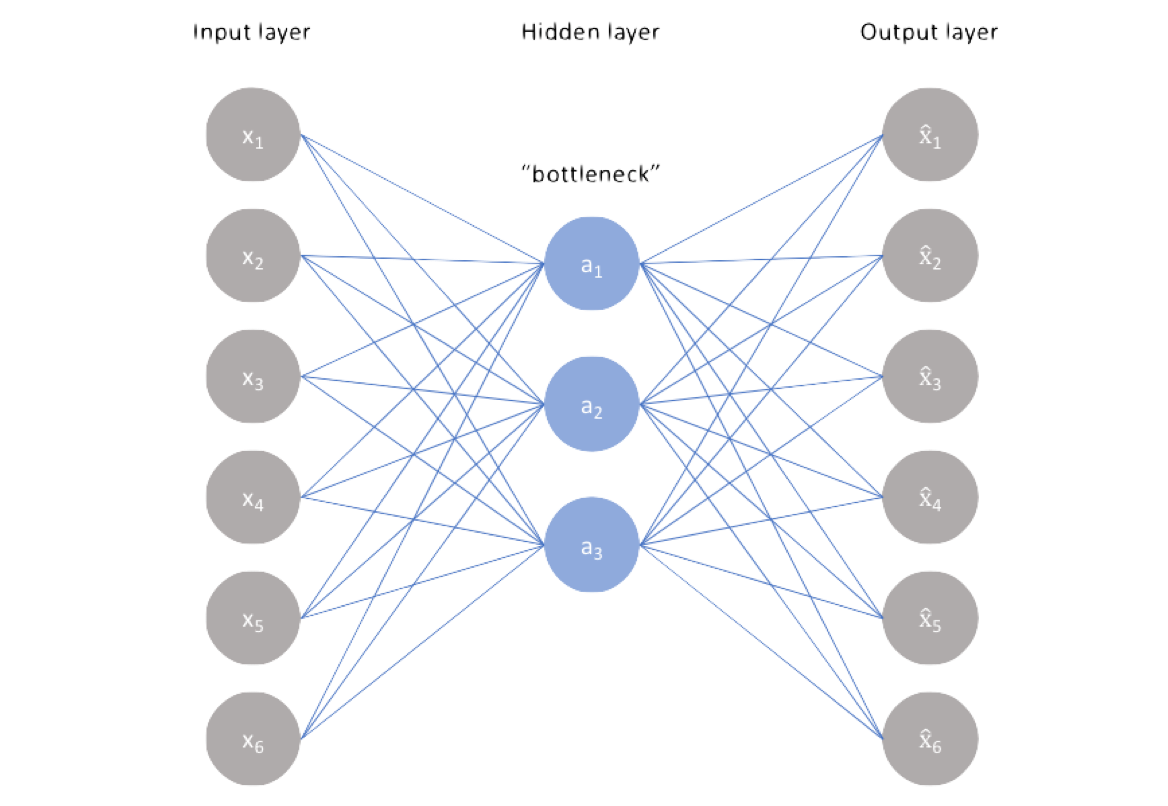
\includegraphics[width=.4\textwidth]{bottleneck.png} \hspace{2em}
		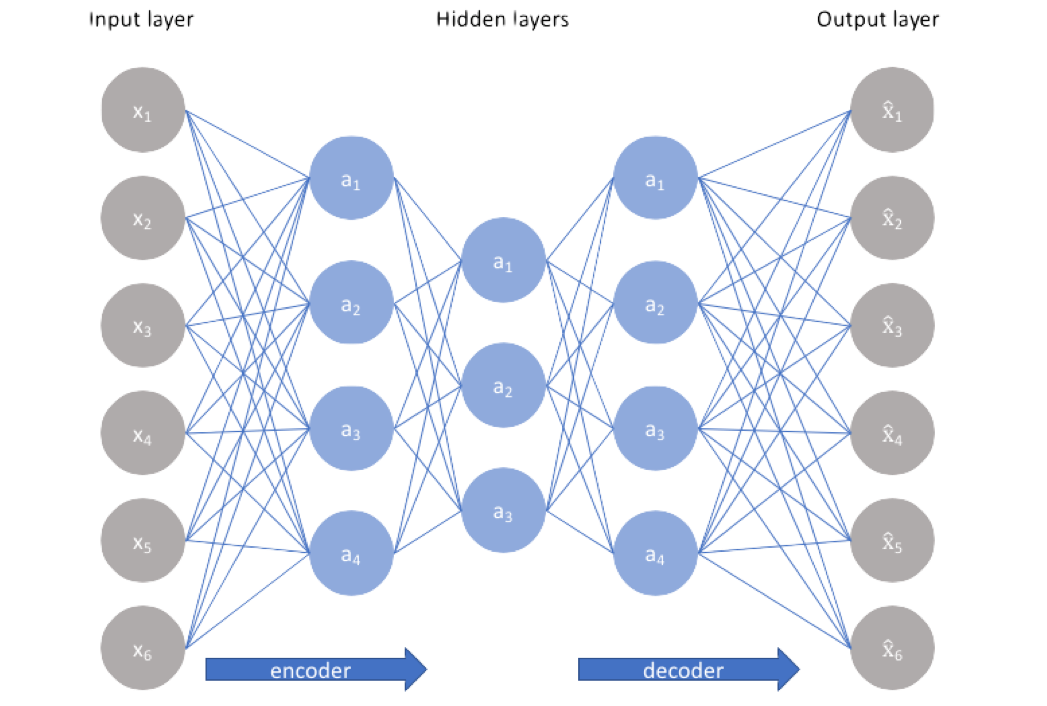
\includegraphics[width=.4\textwidth]{deeper_bottleneck.png}
		
		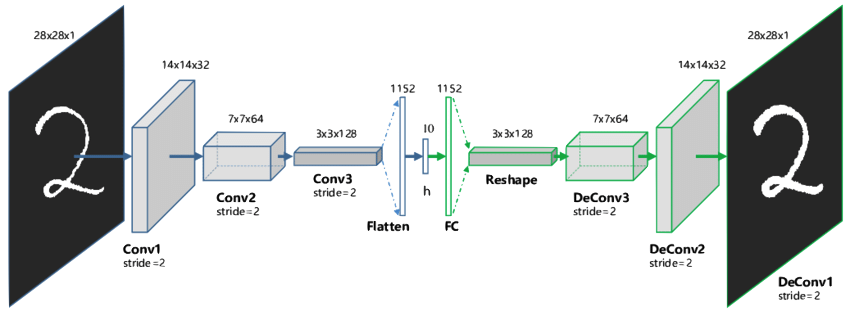
\includegraphics[width=.6\textwidth]{conv_autoencode.png}
	\end{center}	
\end{frame}

\begin{frame}
	\frametitle{autoencoder}
	\small
	Architecture typically split into two parts:
	
	\textbf{Encoder:} $e: \R^d \rightarrow \R^k$
	
	\textbf{Decoder:} $d: \R^d \rightarrow \R^k$
	\begin{align*}
		f(\vec{x}) = \hspace{6em}
	\end{align*}
	\begin{center}
		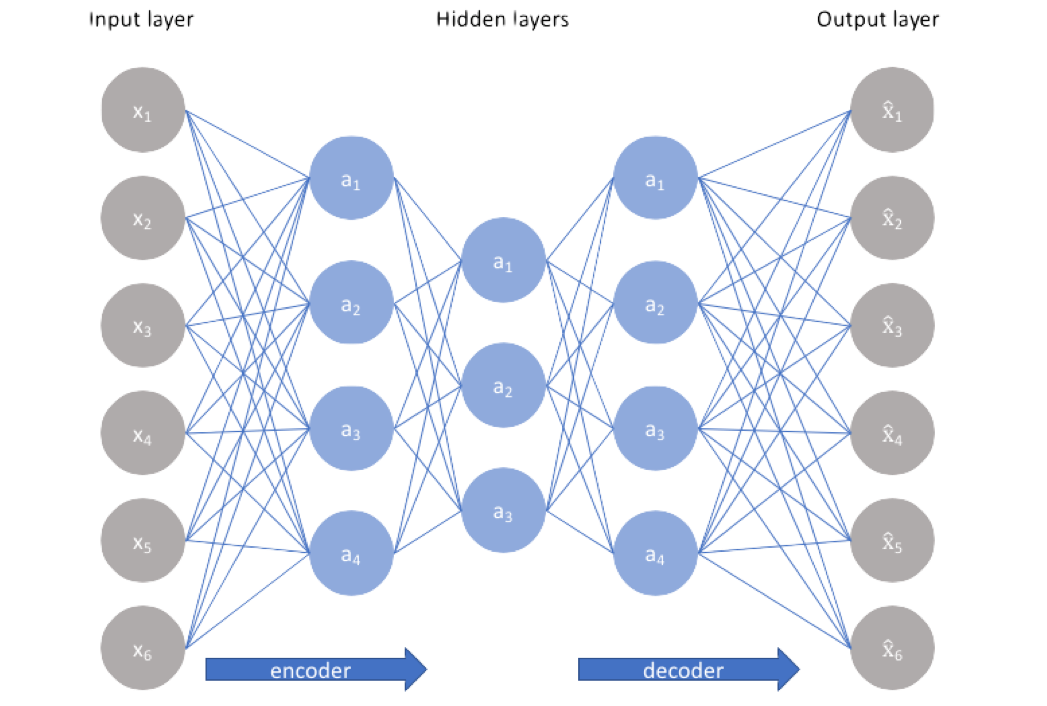
\includegraphics[width=.6\textwidth]{deeper_bottleneck.png}
		
		Often symmetric, but does not have to be.
	\end{center}
	
\end{frame}

\begin{frame}
	\frametitle{autoencoder reconstruction}\small
	\textbf{Example image reconstructions from autoencoder:}
	\begin{center}
		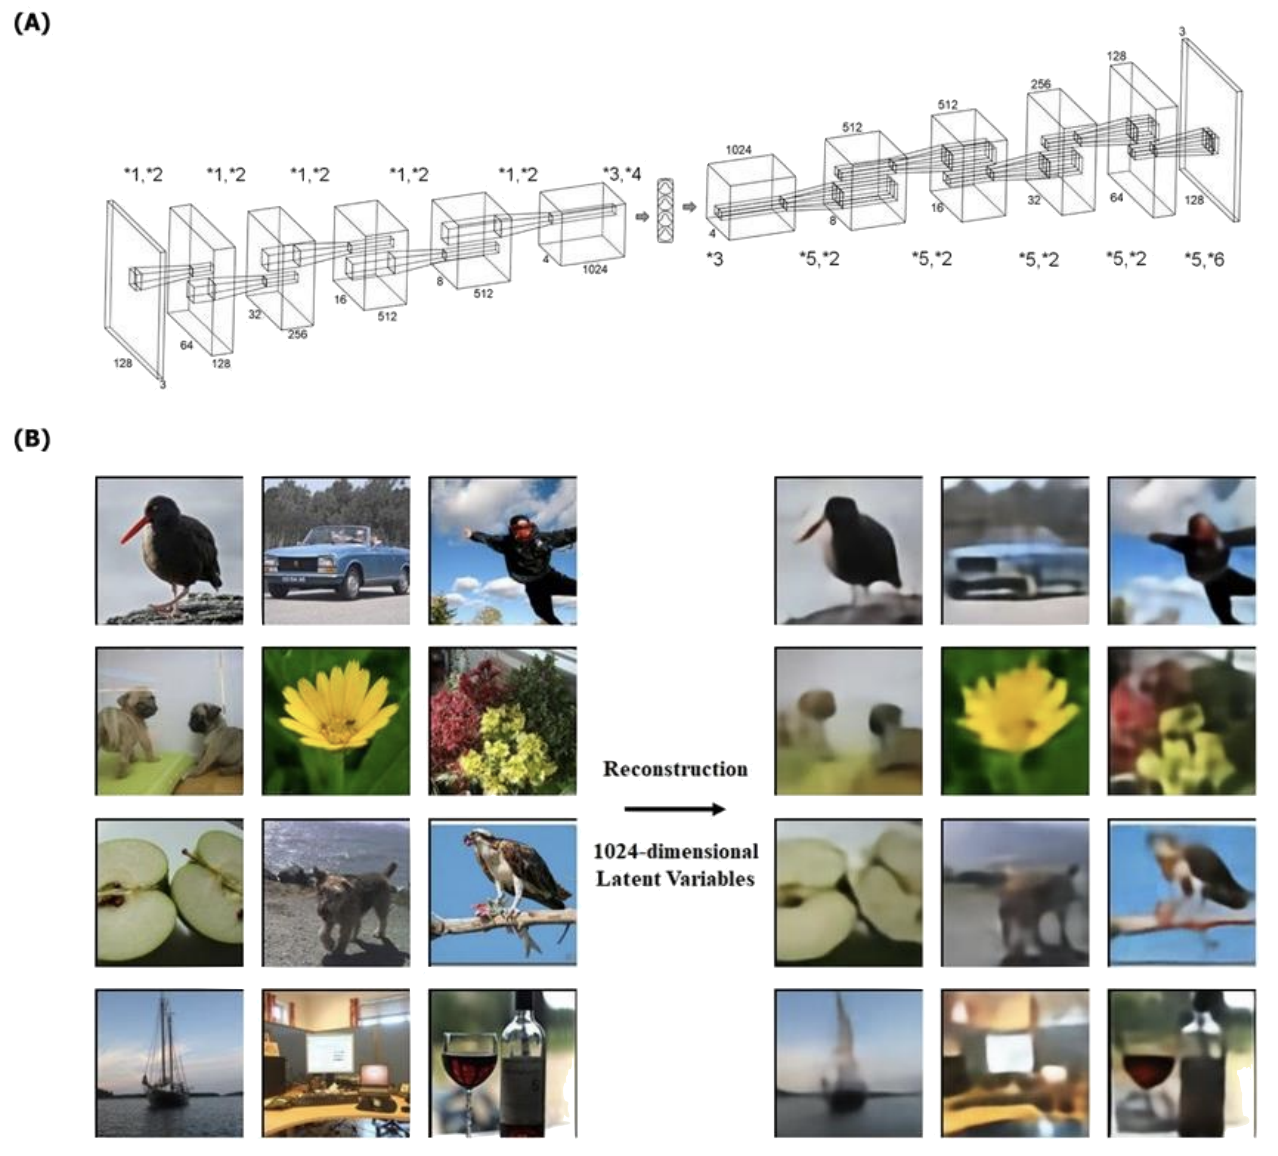
\includegraphics[width=.55\textwidth]{reconstruction.png}
		
		\tiny{\url{https://www.biorxiv.org/content/10.1101/214247v1.full.pdf}}
	\end{center}
	\textbf{Input parameters:} $d = 49152$.\vspace{-.5em}
	
	\textbf{Bottleneck ``latent" parameters:} $k = 1024$.  
\end{frame}


\begin{frame}
	\frametitle{autoencoders for feature extraction}
	At least for now, the best autoencoders do not work as well as for feature extraction as supervised methods. But, they have \emph{many other applications}.
	\begin{itemize}
		\item Image segmentation.
		\item Learned image compression.
		\item Denoising and in-painting.
		\item Image synthesis.
	\end{itemize}
\end{frame}

\begin{frame}
	\frametitle{autoencoders for image segmentation}
	\textbf{Goal:} Learn mask which separates image pixels by what object (foreground or background) that they belong to.
	\begin{center}
		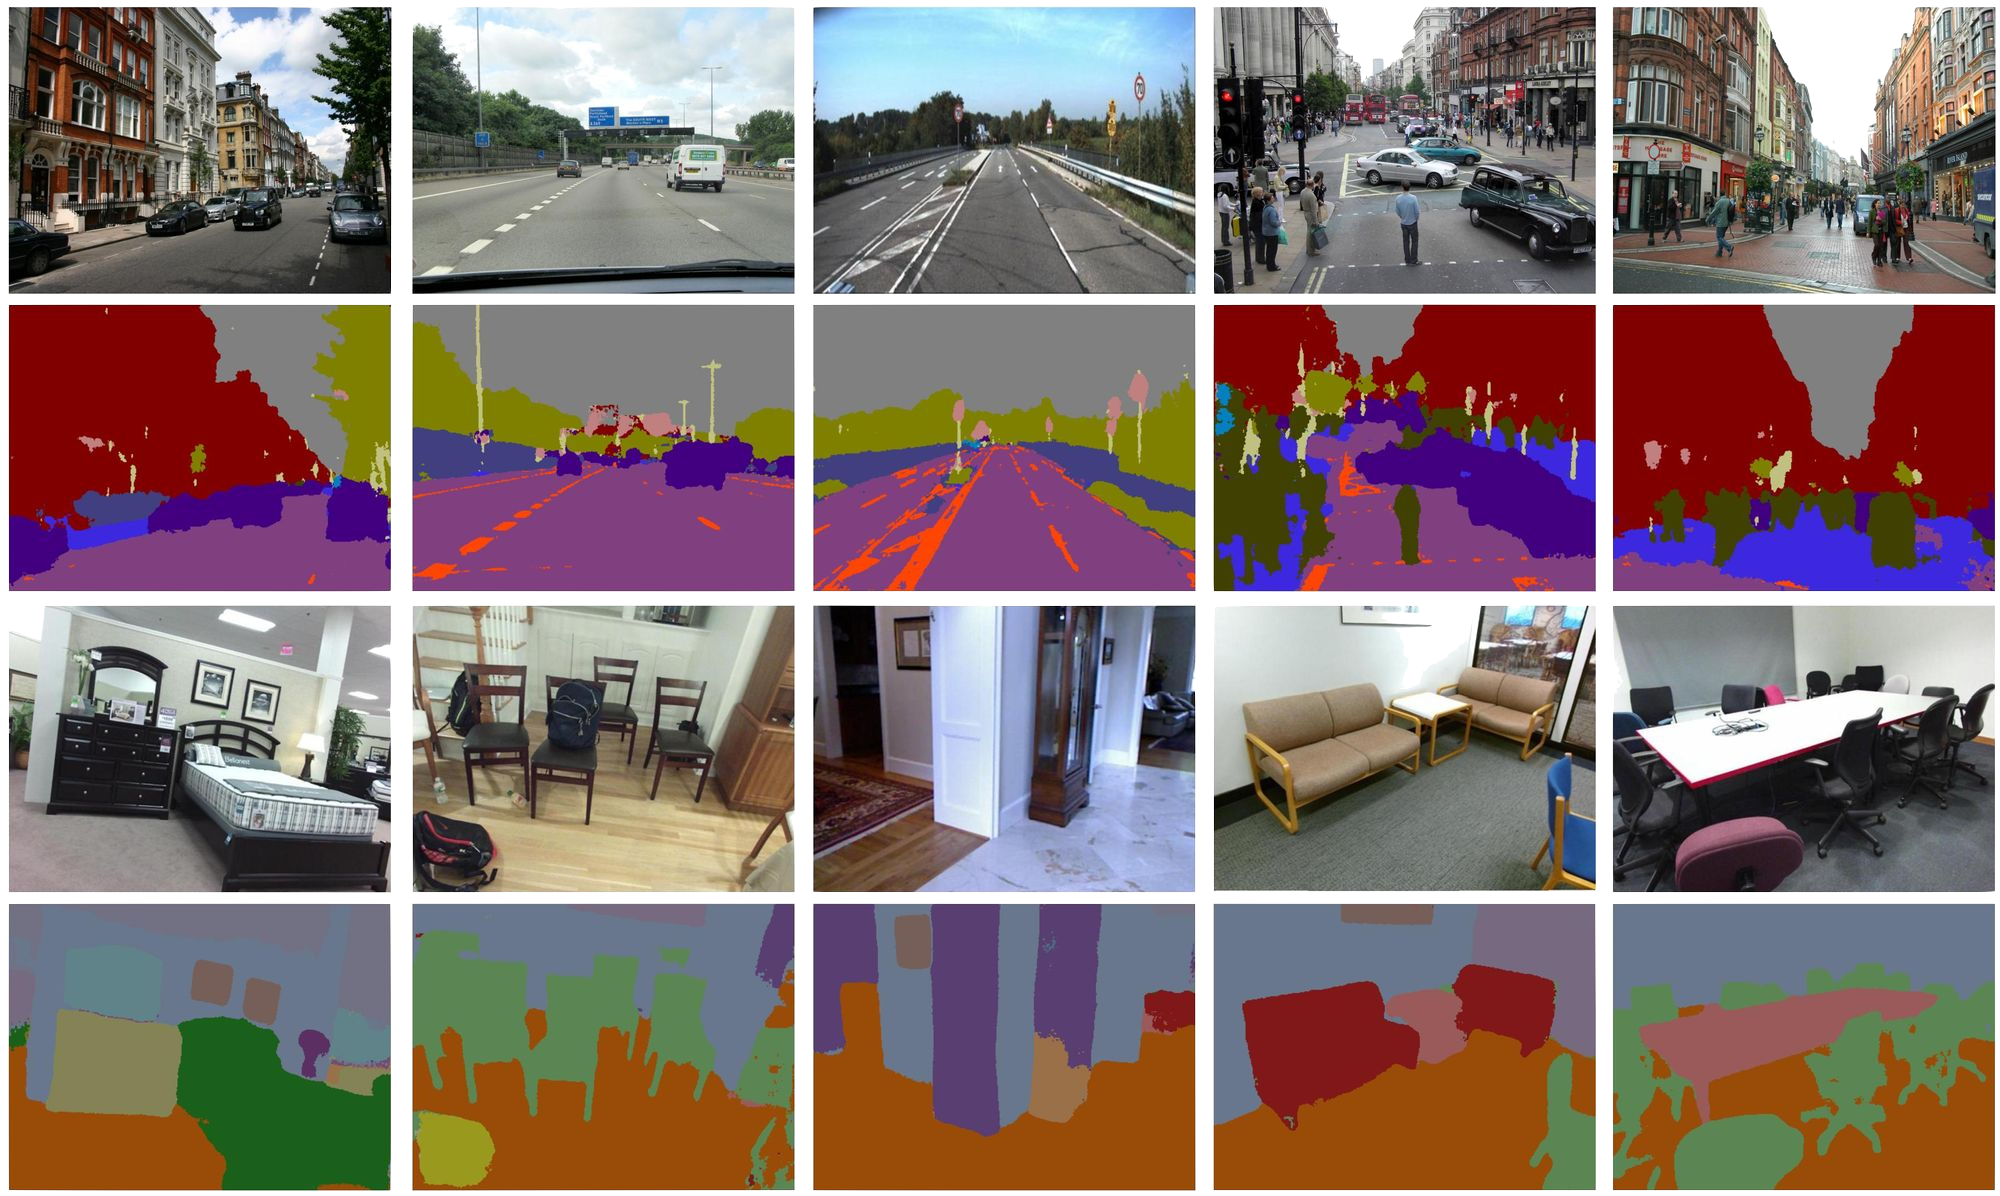
\includegraphics[width=.8\textwidth]{segment.png}
	\end{center}
	First step in \emph{multi-objects classification} and \emph{scene understanding}. Harder than classifying single objects.
\end{frame}

\begin{frame}
	\frametitle{autoencoders for image segmentation}
	\textbf{Change in design:} Input is image $\vec{x}$, output is image $\vec{m}$ that has the same size as $\vec{x}$, but each pixel value is a label for a segmented region.
	\begin{center}
		\includegraphics[width=.8\textwidth]{deepseg.png}
	\end{center}
Now our training process is actually \emph{supervised}, but uses the same structure as an autoencoder.
\end{frame}

\begin{frame}
	\frametitle{autoencoders for image compression}
	Due to their bottleneck design, autoencoders perform \textbf{dimensionality reduction} and thus data compression. 
	\begin{center}
		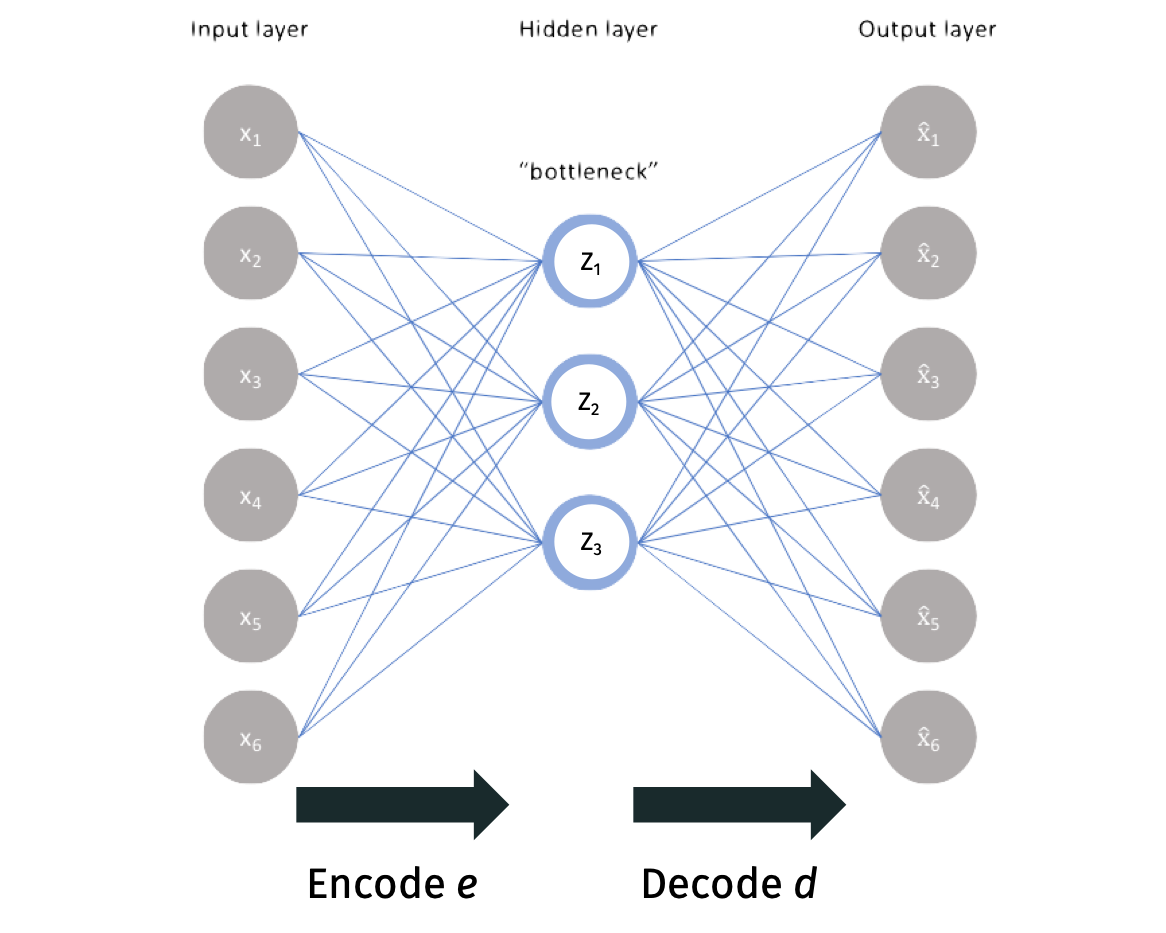
\includegraphics[width=.5\textwidth]{labeled_bottleneck.png}
	\end{center}
Given input $\vec{x}$, we can completely recover $f(\vec{x})$ from $\vec{z} = e(\vec{x})$. $\vec{z}$ typically has many fewer dimensions than $\vec{x}$ and for a typical image $f(\vec{x})$ will closely approximate $\vec{x}$.  
\end{frame}

\begin{frame}
	\frametitle{autoencoders for image compression}
	\small
	The best lossy compression algorithms are tailor made for specific types of data:\vspace{-.5em}
	\begin{itemize}
		\item JPEG 2000 for images
		\item MP3 for digital audio.
		\item MPEG-4 for video.
	\end{itemize}\vspace{-.5em}
	All of these algorithms take advantage of specific structure in these data sets. E.g. JPEG  assumes images are locally ``smooth".
	\begin{center}
		\includegraphics*[width=.3\textwidth]{bwnyu.png}\hspace{4em} \includegraphics*[width=.3\textwidth]{scrambled_nyu.png}
	\end{center}
\end{frame}

\begin{frame}
	\frametitle{autoencoders for image compression}
	\small
	With enough input data, autoencoders can be trained to find this structure on their own.
	\begin{center}
		\includegraphics*[width=.4\textwidth]{compress1.png}\hspace{2em} \includegraphics*[width=.4\textwidth]{compress2.png}
		
		\tiny{``End-to-end optimized image compression'', Ball\'{e}, Laparra, Simoncelli}
	\end{center}
	 Need to be careful about how you choose loss function, design the network, etc. but can lead to much better image compression than ``hand-tuned" algorithms like JPEG.
\end{frame}

\begin{frame}
	\frametitle{autoencoders for image restoration}
	\small
	\begin{center}
		\includegraphics*[width=.6\textwidth]{resto.png}
	\end{center}
\vspace{-1.5em}
	Train autoencoder on \emph{uncorrupted} images (unsupervised). Pass corrupted image $\vec{x}$ through autoencoder and return $f(\vec{x})$ as repaired result.
\end{frame}

\begin{frame}
	\frametitle{autoencoders learn compressed representations}
	\begin{center}
	\textbf{Why does this work?}
	
	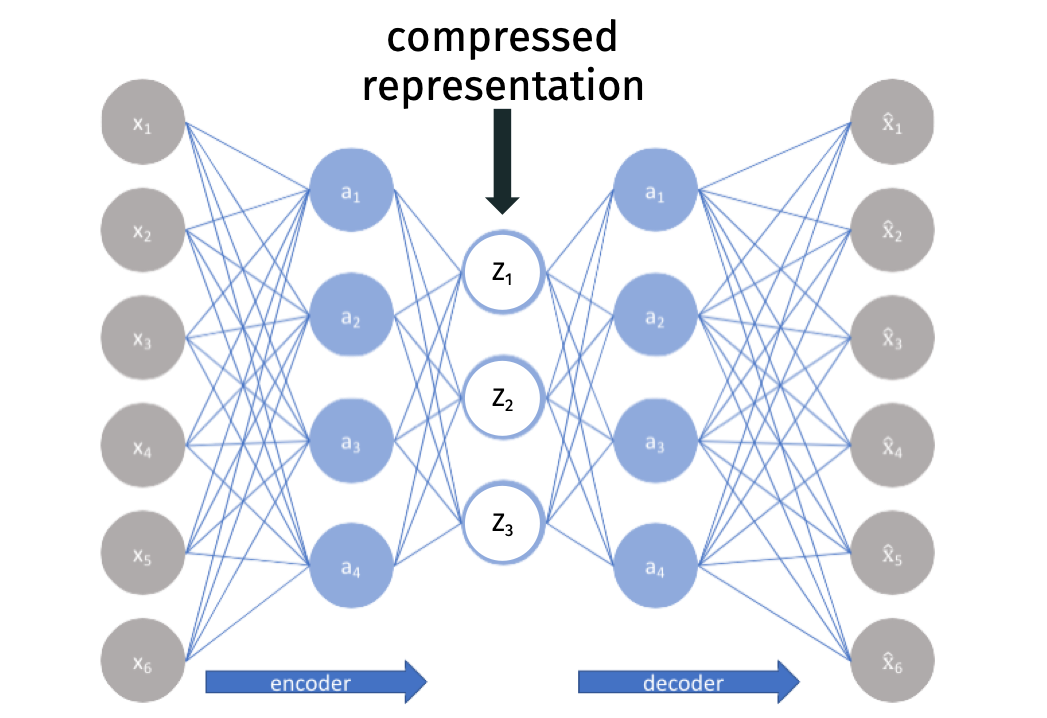
\includegraphics[width=.5\textwidth]{compressed_rep.png}
	\end{center}
Consider $128\times 128 \times 3$ images with pixels values in $0, 1 \ldots, 255$. How many possible images are there?\vspace{.5em}
	
If $\vec{z}$ holds $k$ values between in $0,.1,.2,\ldots, 1$, how many unique images $\vec{w}$ can be output by the autoencoder function $f$?
\end{frame}

\begin{frame}
	\frametitle{autoencoders learn compressed representations}
	\begin{center}
		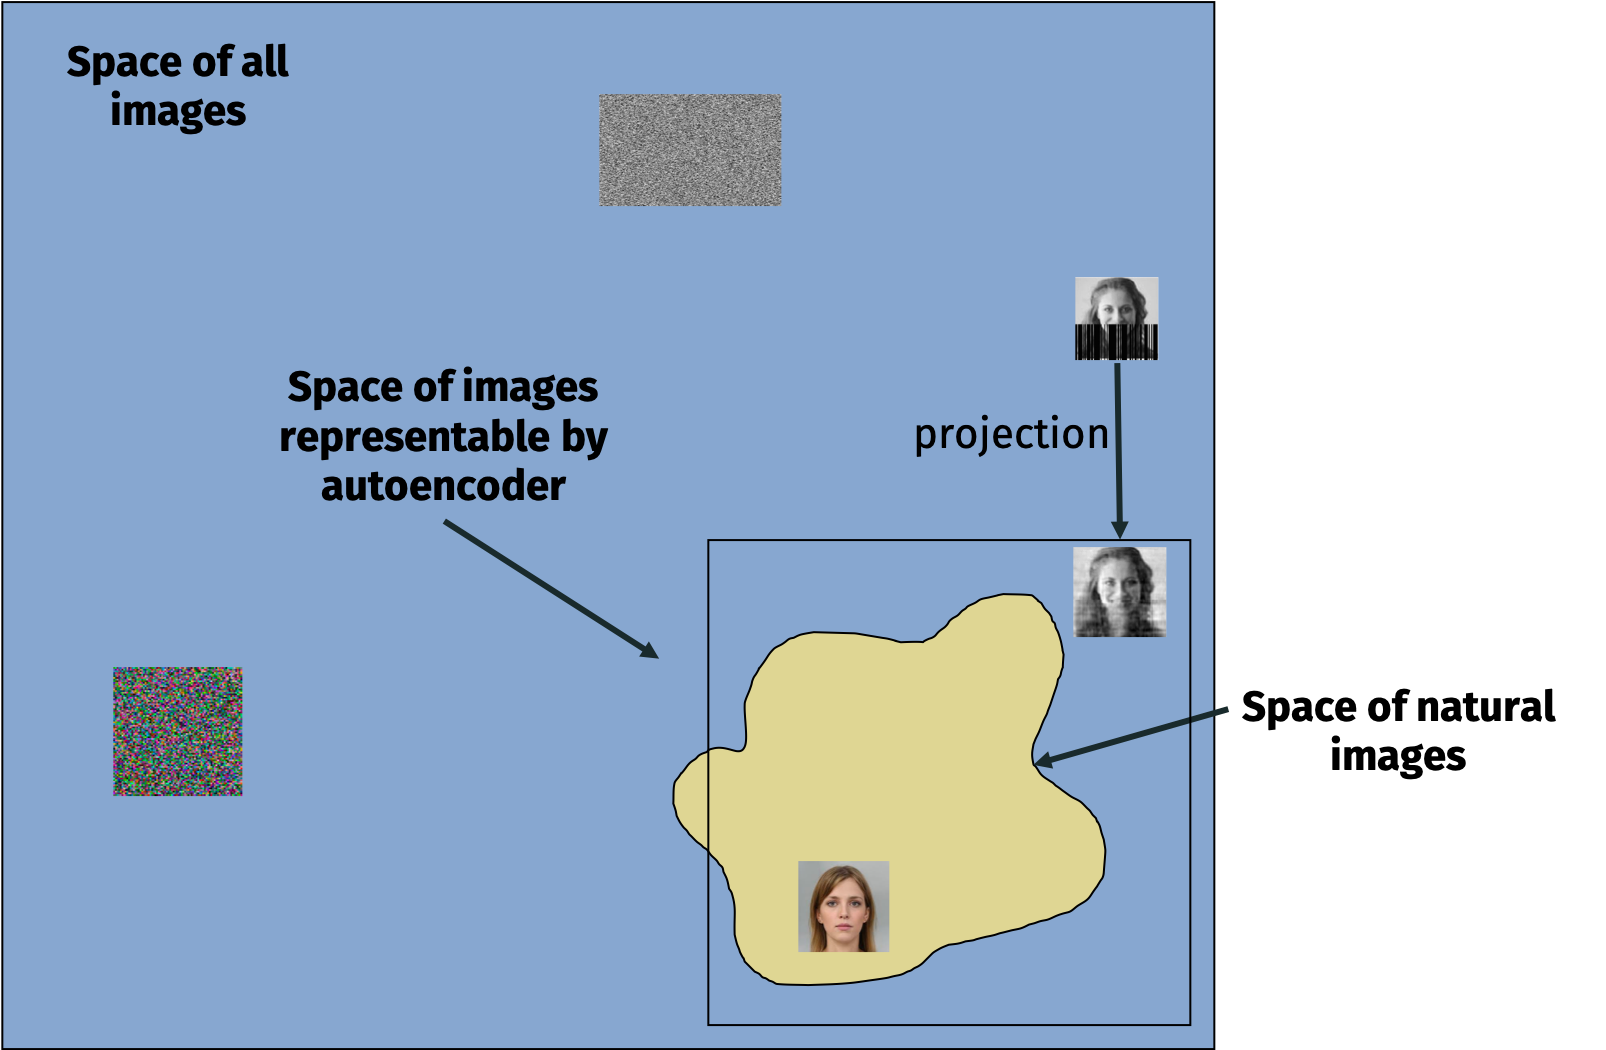
\includegraphics[width=.8\textwidth]{autoencoder_cartoon.png}
	\end{center}
	For a good (accurate, small bottlened) autoencoder, $\mathcal{S}$ will closely approximate $\mathcal{I}$. Both will be much smaller than $\mathcal{A}$. 
\end{frame}

\begin{frame}
	\frametitle{autoencoders learn compressed representations}
	\begin{center}
		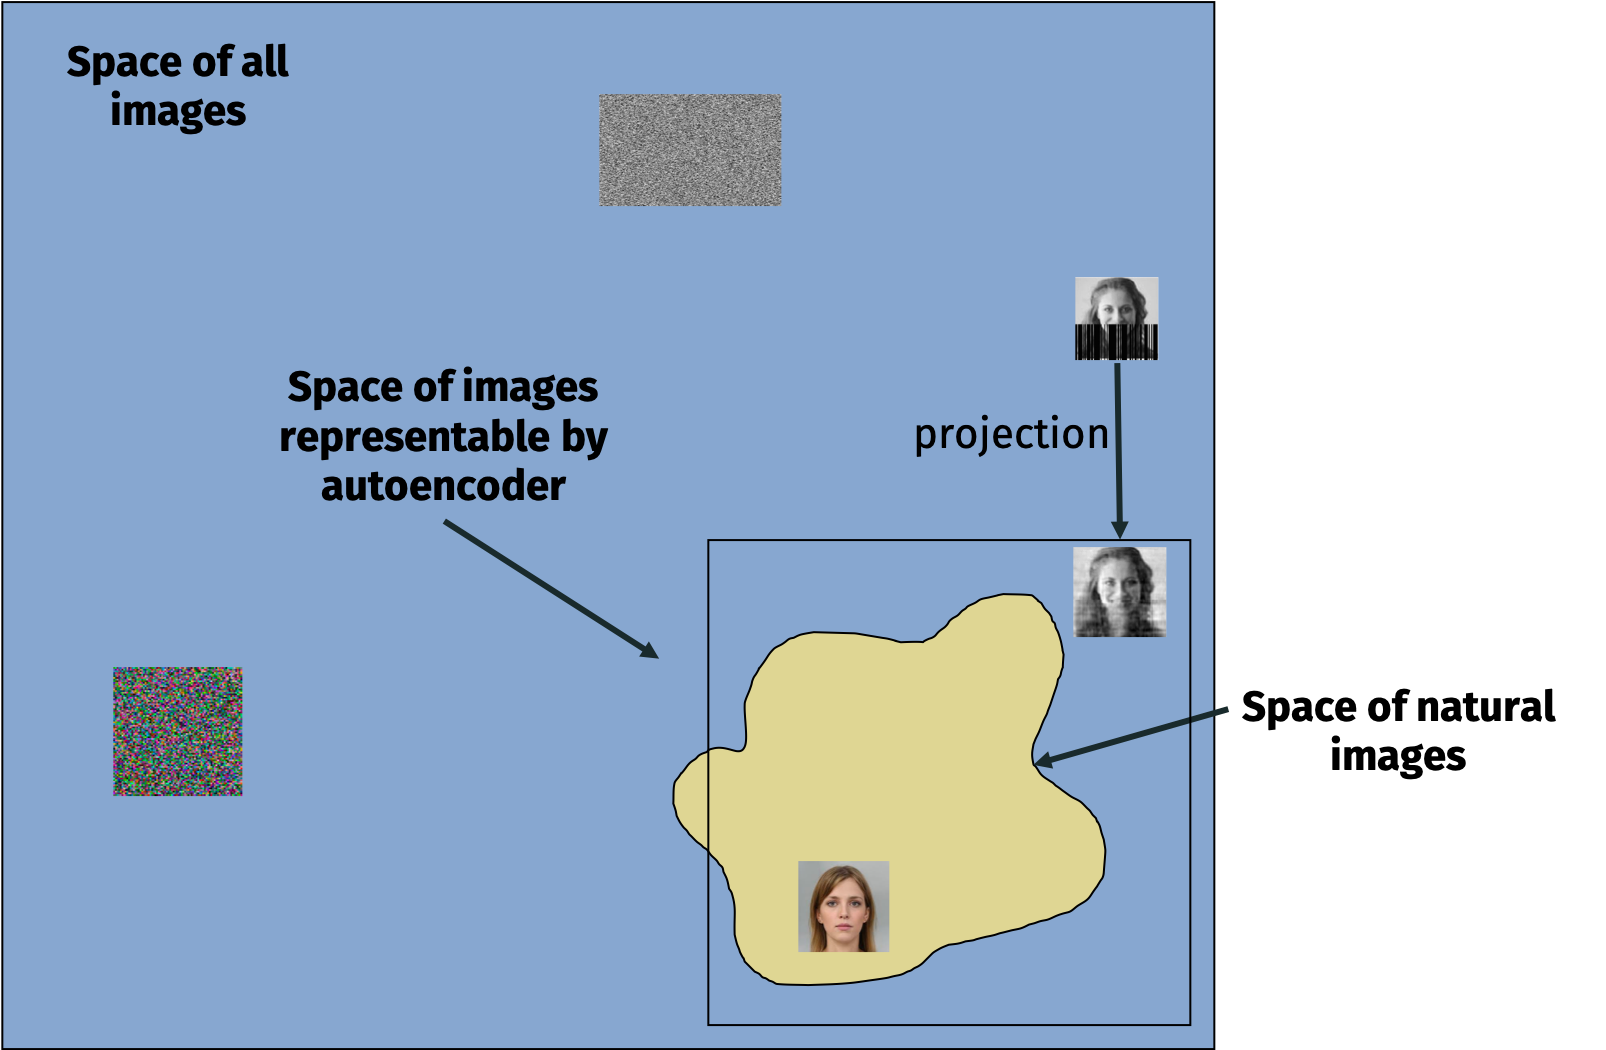
\includegraphics[width=.8\textwidth]{autoencoder_cartoon.png}
	\end{center}
	$f(\vec{x})$ projects an image $\vec{x}$ closer to the space of natural images.
\end{frame}

\begin{frame}
	\frametitle{autoencoders for data generation}
	Suppose we want to generate a random natural image. How might we do that?
	
	\begin{itemize}
		\item \textbf{Option 1}: Draw each pixel in $\vec{x}$ value uniformly at random. Draws a random image from $\mathcal{A}$. Will very likely look like noise.
		\item \textbf{Option 2}: Draw random $\vec{z}\in \R^k$. Let $\vec{x} = d(\vec{z})$ Draws a random image from $\mathcal{S}$. Will look much more like a random image from $\mathcal{I}$.
	\end{itemize}
\end{frame}

\end{document} 



